\documentclass[11pt, a4paper, twoside]{article}
\usepackage[utf8x]{inputenc}
\usepackage[spanish]{babel}
\usepackage{times}
\usepackage[T1]{fontenc}
\usepackage{anysize}
\usepackage{tabu}
\usepackage{pdfpages}
\usepackage{fancyhdr}

% Penaliza los guiones a final de línea
\hyphenpenalty = 9999

\marginsize{3cm}{2cm}{2cm}{2cm}

% Indicador completo en lugar de página
\fancyhead[LR]{}
\fancyfoot[C]{{\ttfamily RTF PKT:CU \quad \thepage}}

\renewcommand*{\headrulewidth}{0pt}
\pagestyle{fancy}

\renewcommand*{\appendix}{\setcounter{section}{0}\setcounter{subsection}{0}\renewcommand*{\thesection}{Anexo \Alph{section}}}

\newcommand*{\PKT}{P\lower2pt\hbox{K}\kern-2pt\raise2pt\hbox{T}\kern-2pt}

% Comando para indicar los problemas
\newcommand{\problema}[2]{\begin{description} \item[Exposición] #1 \item[Resolución] #2 \end{description}}

\begin{document}

	% Título
	\begin{center}
		\scshape \large Acta de la Revisión Técnica Formal \textit{Casos de uso} - \PKT\ \vspace{.5cm}
	\end{center}

	Reunidos de una parte Jaime Dan Porras, Alejandro Villarín Prieto e Ignacio Iker Prado Rujas en representación de \PKT\ en calidad de autores del documento y de la otra Rubén Rafael Rubio Cuéllar y Juan Andrés Claramunt Pérez de la parte revisora, el \textsc{Grupo Diedral}, se procede a la puesta en común de la Revisión Técnica Formal del documento \textsc{Casos de uso} perteneciente a \PKT\ . \\

	El equipo revisor presenta un documento, anexo al presente, con sus conclusiones previas. \PKT\ defiende su documento y el \textsc{Grupo Diedral} expone los problemas encontrados, como se refiere en el~\ref{acta:acta}. Por lo cual el equipo revisor concluye:

\begin{quotation} \itshape
	El documento adolece de ciertos problemas sistemáticos, principalmente la ausencia de un formato propio de casos de uso (falta de precondiciones, entradas\ldots) y la nada conveniente inclusión en cada caso del inicio y cierre de sesión, así como de la secuencia\break necesaria para llegar hasta él. Estos defectos si bien son serios también parecen ser\break fácilmente subsanables pues, la dificultad de establecimiento de los casos de uso radica más bien en la comprensión de las necesidades del usuario y la especificación coherente de las mismas, lo cual se considera logrado. En este sentido también merece atención la\break ausencia de detalle y la presencia de ciertas inconsistencias en algunas partes \mbox{localizadas} del documento que han sido advertidas y podrán ser corregidas directamente. Esta\break evaluación pone en perspectiva un trabajo extenso pero rutinario y asentado en unas bases de suficiente firmeza.
\end{quotation}


\noindent
En virtud de lo anterior, el documento se declara \textsc{rechazado}.\\

	Ambas partes expresan su conformidad con lo referido en este acta en Madrid, a \today.

\begin{flushleft}
	Los asistentes,
\end{flushleft}

\vspace{1cm}

	% Espacio para firmar
	\begin{tabu} to .9\linewidth {X[1,c] X[1, c] X[1, c]}
		Jaime Dan Porras & Alejandro Villarín Prieto & Iker Ignacio Prado Rujas
	\end{tabu}

	\vfill

	\begin{tabu} to .9\linewidth {X[1,c] X[1, c]}
		Rubén Rafael Rubio Cuéllar & Juan Andrés Claramunt Peréz
	\end{tabu}
	
	\vfill
	{\itshape A continuación se incluye el acta detallada de la reunión: }

	% Acta detallada de la reunión
	\newpage
	\appendix
	\section{Acta detallada de la reunión}	\label{acta:acta}

		Se exponen los temas tratados por orden de aparición:

	\begin{enumerate}
		\renewcommand*{\theenumi}{P\arabic{enumi}}
		
		\item \problema{La especificación de los casos de uso no se ajusta al esquema de los apuntes. En particular se hecha en falta el epígrafe de precondiciones que quedan incluidas, cuando quedan, de forma extraña en el propio ``curso típico de eventos''.}{Se revisarán todos los casos de uso para que se ajusten a este esquema.}
		\item \problema{Casi todos los casos de uso comienzan con el usuario registrándose en el sistema y acaban cerrando la aplicación. Esto parece demasiado drástico.}{\PKT\ está de acuerdo y lo cambiará en todos sus casos de uso.}
		\item \problema{La secuencia de acciones de muchos casos de uso relata el recorrido que ha hecho el usuario hasta llegar a la función, lo cual es irrelevante desde el punto de vista del caso de uso.}{Se tratará de nuevo en todos los casos de uso.}
		\item \problema{Se utilizan muchos términos tecnológicos como ``pestaña'', ``clica'', ``tacha'', ``tick'', ``pulsar'', ``botón'', ``cuadro de texto'', ``pinchar'' o ``ventana'' a lo largo de todo el documento.}{Estos términos serán eliminados del documento.}
		\item \problema{En general no queda claro por qué algunas secuencias son alternativas y no típicas.}{Se aclararán los motivos por los que una secuencia es alternativa en un caso de uso.}
		\item \problema{Faltan algunas tildes (están marcadas en el documento).}{Se corregirán.}
		\item \problema{Errores concretos por inconsistencias que se detallan en el anexo.}{Se corregirán en la siguiente revisión.}
		\item \problema{Que el ``extracto'' sea una ``parte'' del documento puede resultar excesivo. Se puede hacer {\ttfamily \textbackslash chapter$^{*} \{Extracto \}$} o usar el entorno {\ttfamily abstract}
.}{Se tendrá en cuenta cuando se revise la organización del documento.}
		\item \problema{En el caso de uso 1.1. se dice ``Actores: Todos'' pero los actores no han sido presentado previamente.}{Se presentarán previamente.}
		\item \problema{En el caso 1.2. los campos no quedan muy claros, especialmente el de historial. En los cursos alternativos aparece que si no encuentra el nombre pregunta por el NIF; es decir, que si quieres buscar por el NIF tienes que escribir un nombre falso (anteriormente se usa DNI en lugar de NIF).}{\PKT\ acuerda cambiarlo.}
		\item \problema{Caso 1.3: cuando el actor se equivoca al rellenar un campo, ¿el programa le informa de la causa del error?. Caso 2.5: ``los campos que sean necesarios'' no es preciso.}{\PKT\ considera que no tiene excesiva importancia.}
		\item \problema{Casos 1.7, 1.14, 1.27, 2.11: están incompletos.}{Se completarán los casos de uso indicados, o se moverán a secundarios.}
		\item \problema{Caso 1.11: ejemplo de explicación de cómo se ha llegado hasta allí no conveniente. La interacción queda fijada como de tipo pregunta-respuesta por la redacción del curso típico.}{Se corregirá en una posterior revisión.}
		\item \problema{Caso 1.12: el título ``anular reserva'' no aclara, sin mirar al resto del documento, si se trata de una reserva de hotel de restaurante o ambas (igual con los siguientes). ¿Qué pasa si no hay reservas?}{\PKT\ acuerda solucionar la ambigüedad de alguna forma.}
		\item \problema{Caso 1.13: se afirma que ``el programa manda el pedido a la cocina'', ¿cómo?. En el epígrafe 5 no queda muy claro qué es la carta y cómo se añaden o eliminan ingredientes. En los casos de contabilidad falta detalle. Caso 1.24: se refieren las ``características de las habitaciones'', ¿cuáles son?. Caso 1.25: está escrito ``se guarda toda la información de la reserva'', ¿qué información? Igualmente ``los campos a completar''. Caso 2.4: ¿de qué datos se compone un currículum?.}{\PKT\ opina que no son importantes esos detalles, en contra de la opinión del \textsc{Grupo Diedral}.}
		\item \problema{Caso 1.15: se dice ``siempre que no haya empezado a prepararse'', ¿el programa sabe cuándo un plato está preparándose?}{Se acuerda que \PKT\ solucionará de alguna forma el problema, o eliminará el caso de uso.}
		\item \problema{Caso 1.18 y 1.19: los nombres de los diagramas no coinciden con los nombres de los casos de uso en el texto del documento.}{Los autores se comprometen a modificar los diagramas.}
		\item \problema{Caso 1.26: se llama ``ver reservas'' que no aclara por sí mismo si se trata de reserva de hotel o de restaurante. Además falta el correspondiente a reservas de restaurante. ``Se muestran la lista de reservas''.}{Se admite para ser corregido.}
		\item \problema{Caso 2.6: la ``visión general'' y el curso ``típico de los eventos'' son casi lo mismo.}{Se cambiará la visión general para que no sea tan detallada.}
		\item \problema{Caso 2.9: que una cantidad de algún elemento de las existencias no varíe, ¿no es típico? El ``introducir Intro'' induce a pensar que se tiene una interfaz de consola (desde luego es una referencia tecnológica indeseada). En cambio, marcar la opción ``Guardar y salir'' sugiere una interfaz gráfica.}{Estos detalles de bajo nivel serán sustituídos por una descripción de más alto nivel.}
		\item \problema{Caso 2.10 (añadir plato): la interacción es controlada rígidamente por el programa. ¿Qué son los ingredientes? ¿Están prefijados? Esa duda se resuelve en los cursos alternativos pero se introduce una base de datos: ¿es modificable? ¿existe un caso de uso para ello?.}{Se corregirá el caso de uso para que puedan introducirse manualmente los ingredientes y no tengan por qué estar prefijados. Se añadirán casos de uso secundarios que permitan editar la base de datos de ingredientes.}
		\item \problema{Caso 2.10 (borrar plato): se afirma que el plato borrado queda almacenado en una base de datos para su posible uso posterior, pero no se explica cómo se recupera.}{Se elimina esa afirmación del caso de uso.}
		\item \problema{Caso 2.10: deberían ser más de un caso de uso.}{Se acuerda separarlos y añadir los que sean necesarios.}
		\item \problema{Parte de lo dicho de algunos casos particulares se puede aplicar en otros.}{Se le dará una pasada al documento corregido y se modificarán los casos de uso en los que esté indicado algún error de los que se han aceptado corregir en los puntos anteriores.}
	\end{enumerate}

	\vfill
	{\itshape A continuación se incluye el anexo previo elaborado por el equipo revisor: }

	% Incluye el anexo del otro grupo
	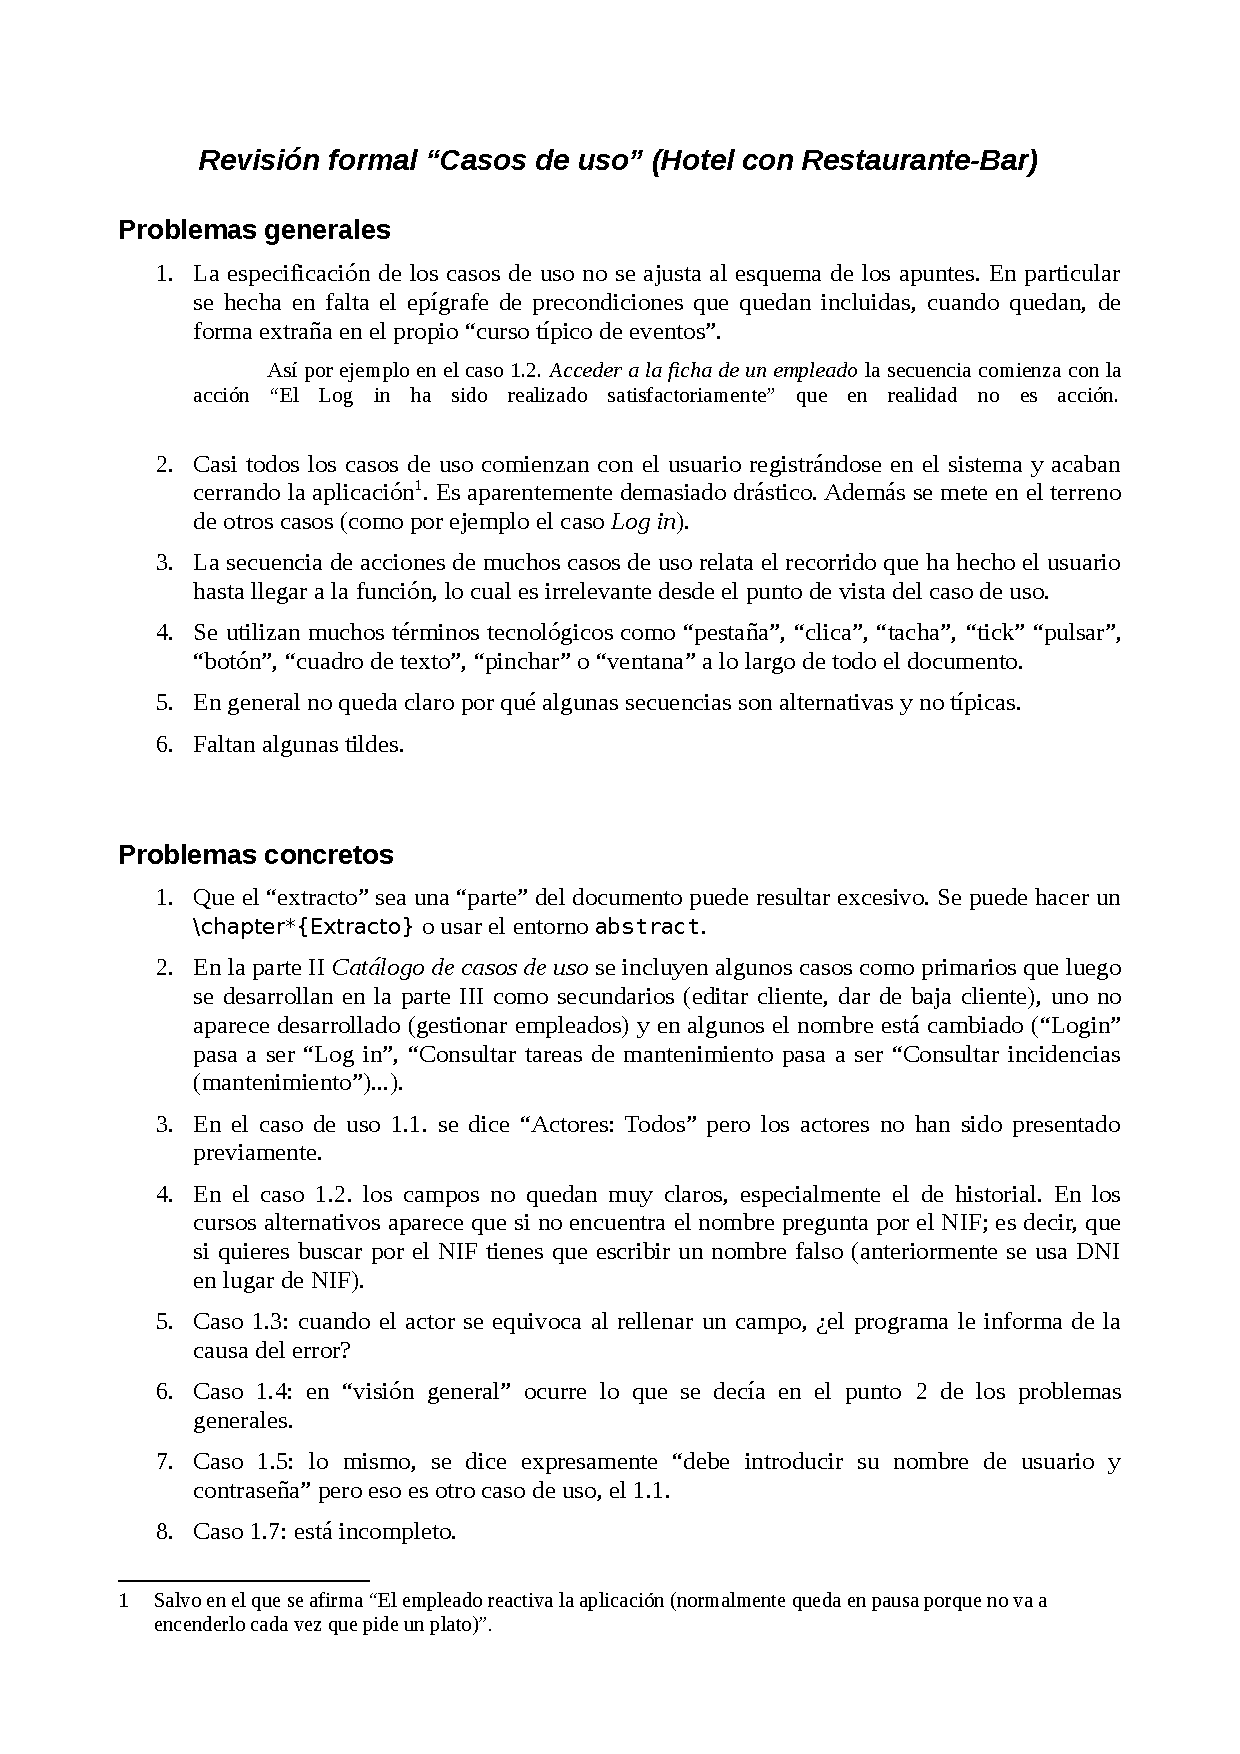
\includepdf[pages=1-2, pagecommand={}]{casosdeuso_pkt_anexo.pdf}
\end{document}
